\section{RSI Across Applications}
\label{sec:rsi-applications}


\begin{figure*}[!t]
    \centering
    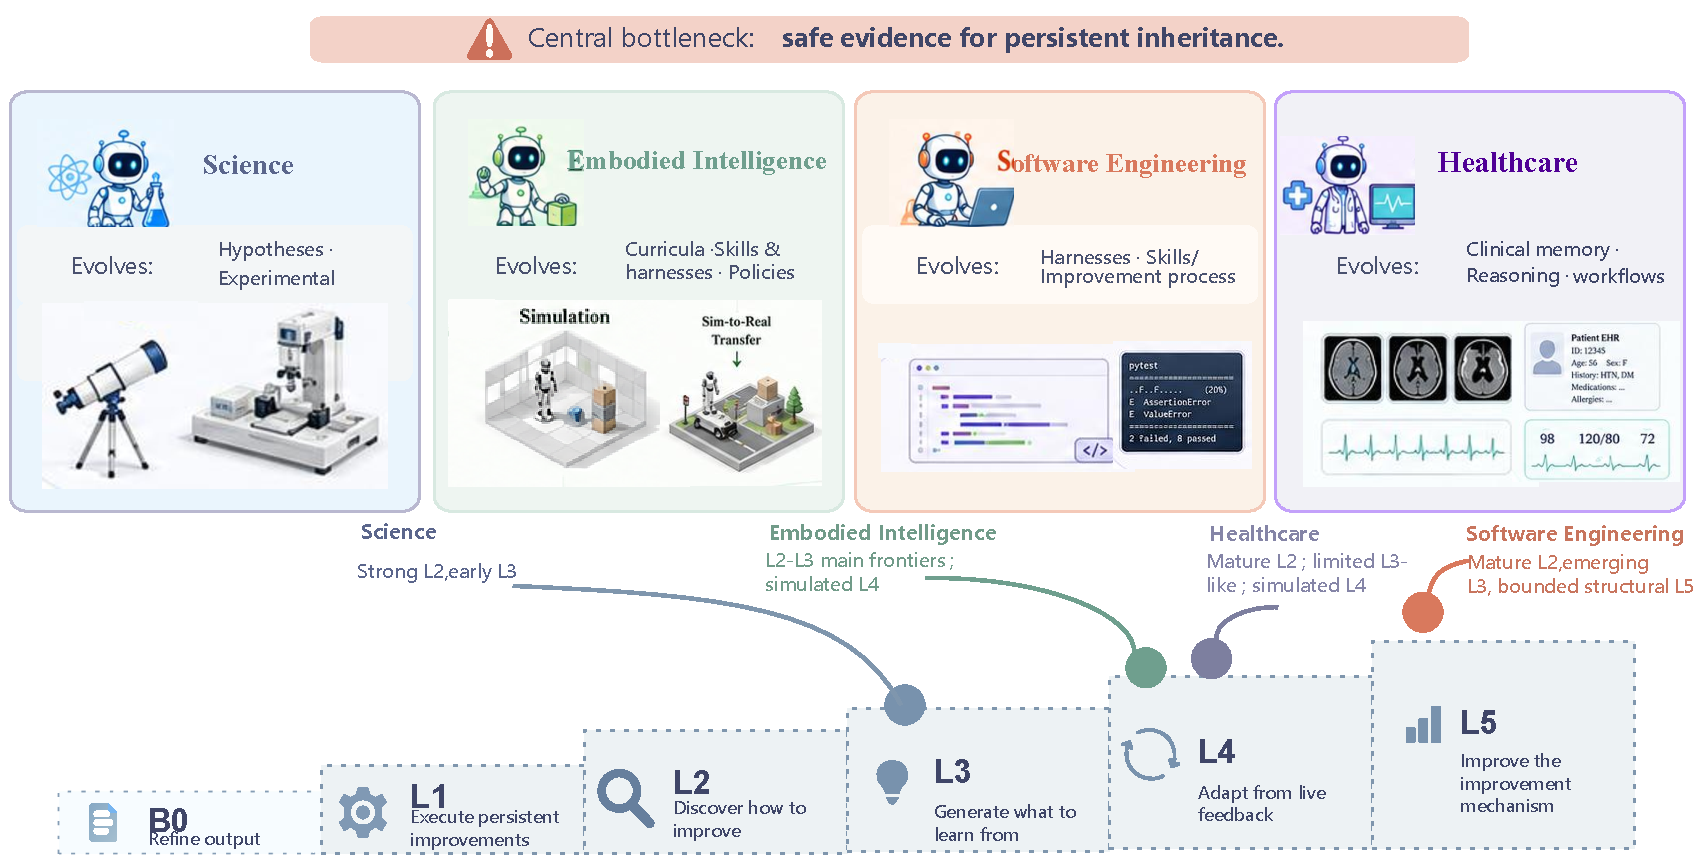
\includegraphics[width=1\linewidth]{figures/part2-v3.pdf}
    \caption{Application regimes differ mainly in the kind of feedback needed to validate and inherit an improvement.}
    \label{fig:rsi-applications}
\end{figure*}

Building on the B0--L5 taxonomy, this section summarizes how recursive self-improvement is instantiated under four domain-specific feedback regimes, including science, embodied intelligence, software engineering, and healthcare. Across these regimes, repeated refinement of an external artifact is insufficient: the feedback must produce a persistent change to the AI system that is reused in later tasks. Current evidence is therefore strongest for bounded, component-level improvement, whereas adaptation of the improvement mechanism itself remains rare.
A detailed review of the evolving components, supporting evidence, and remaining limitations in each application is provided in Appendix~\ref{app:rsi-applications}. 

\subsection{S1: RSI for Science}
\label{subsec:science-main}

Science is a consequential setting for RSI because progress depends not only on solving individual problems, but also on improving how future hypotheses are generated, tested, and revised. Its characteristic loop uses experimental evidence or falsification to update the AI4Sci system: a research agent proposes hypotheses, executes computational or physical experiments, attributes the observed outcomes, and retains validated changes to its generation strategy, tools, skills, memory, or scaffold. HypoForge~\cite{qian2026hypoforge}, for example, distills critiques and execution outcomes into reusable skills for hypothesis generation and testing. Test-Time Tool Evolution~\cite{lu2026tool} synthesizes and validates executable scientific tools for reuse, while DrugSAGE~\cite{zhang2026drugsage} transfers verified modeling procedures and error-recovery strategies across tasks. SIA~\cite{hebbar2026sia} extends the editable surface to agent scaffolds, tools, search logic, and model weights. These systems demonstrate persistent improvement of scientific-agent components, but their evaluators, update-selection rules, and promotion criteria remain largely fixed; improving a molecule, equation, or hypothesis alone therefore remains RSI-adjacent rather than evidence that the scientific agent has improved itself.

\subsection{S2: RSI for Embodied Intelligence}
\label{subsec:embodied-main}

Embodied intelligence grounds improvement in physical interaction and causal feedback. An embodied RSI loop selects or generates experience, executes a policy, evaluates the resulting trajectory, and commits validated updates to the policy, world model, skill library, harness, or curriculum used in subsequent interactions. POET~\cite{wang2019poet} co-evolves environments and agents so that newly generated challenges expose and extend current capabilities. Voyager~\cite{wang2023voyager} converts successful behaviors into an executable skill library that supports later exploration, and World-VLA-Loop~\cite{liu2026worldvlaloop} alternates between improving a world model from policy failures and optimizing the policy in the refined model. Together, these works move beyond within-episode correction toward persistent agent--environment co-adaptation. However, embodied experience is endogenous to the current policy, failures are difficult to attribute across perception, planning, control, and hardware, and real-world trials are costly and unsafe to reset. Most reported loops consequently rely on simulation or externally specified rewards, evaluators, interfaces, and safety constraints, leaving autonomous real-world validation and evolution of the embodied improver unresolved.

\subsection{S3: RSI for Software Engineering}
\label{subsec:software-main}

Software engineering offers unusually direct feedback because both the developed artifact and the coding agent can be represented, executed, versioned, and rolled back as code. Its RSI loop proceeds from a development challenge to an agent-level modification, repository-grounded execution, regression-aware selection, and versioned inheritance. SWE-Exp~\cite{chen2026sweexp} extracts lessons from successful and failed issue-resolution trajectories for reuse across repositories. Self-Harness~\cite{zhang2026selfharness} uses execution traces to propose modifications to its own harness and retains them only after regression testing. Darwin G\"odel Machine~\cite{zhang2026dgm} broadens this process by maintaining lineages of self-modifying coding agents and selecting variants according to executable task performance, thereby allowing accepted descendants to become the starting points for further improvement. These systems provide some of the clearest evidence of persistent source-, harness-, and experience-level evolution. Nevertheless, repository tests are incomplete proxies for user intent, security, maintainability, and descendant quality; benchmarks, utility functions, sandboxes, and selection rules also remain externally defined. Software-engineering RSI is therefore comparatively auditable, but still bounded by a fixed outer improvement contract.

\subsection{S4: RSI for Healthcare}
\label{subsec:healthcare-main}

Healthcare requires RSI to be grounded in longitudinal feedback from experts, clinical guidelines, diagnostic evidence, and patient outcomes. A clinical RSI loop performs a task, obtains validated feedback, updates a persistent component such as memory, reasoning policy, tool repertoire, or workflow, and reuses the approved update across later cases. MedAgent-Zero in Agent Hospital~\cite{li2024agenthospital} stores successful cases and derives reusable diagnostic rules from failures. EvoClinician~\cite{he2026evoclinician} uses process-level grading to revise how an agent acquires and integrates diagnostic evidence, while MACRO~\cite{fan2026macro} composes verified medical-imaging trajectories into reusable tools. HealthFlow~\cite{zhu2026healthflow} similarly retains validated safeguards, workflows, and code from completed health-data analyses. These approaches show how clinical experience can improve future agent behavior without necessarily changing foundation-model weights. Their evidence, however, remains dominated by simulated or retrospective settings, while real outcomes are delayed, heterogeneous, and confounded. Persistent clinical updates must therefore remain provenance-aware, population-specific, prospectively monitored, reversible, and subject to expert and institutional approval; autonomous evolution of the clinical improver is not yet established.
